\documentclass[a4paper,10pt]{scrartcl}

\usepackage{units}
\usepackage{mathtools}
%\usepackage{a4wide}
\usepackage{bbm}
\usepackage{amssymb}
\usepackage{amsthm}
\usepackage{amsmath}
\usepackage{graphicx, enumerate}
\usepackage{psfrag}
\usepackage[matrix, arrow, curve]{xy}
\usepackage{array,tabularx}
%\usepackage[square, comma, numbers]{natbib}
\usepackage[unicode, a4paper]{hyperref}
\usepackage{subfigure}
\usepackage{algorithm2e}
\usepackage{url}
\usepackage{mathtools}
\usepackage{pgfplots}
\usepackage{siunitx}

\newcounter{myFCounter}[section]
\newcommand{\myFigure}[3]{%
    \begin{center}\begin{minipage}[t]{\columnwidth}%
    \begin{center}\refstepcounter{myFCounter}\vspace{1ex}%
    \includegraphics[width=#1\columnwidth,keepaspectratio]{#2}\ \\%
     Abb. \arabic{myFCounter}:\ \rm #3 
    \vspace{1ex}\end{center}%
    \end{minipage}\end{center}}
    \newcommand\myColumnSep[1]{%
\setlength{\columnsep}{#1}%
}

\newcommand{\inner}[2]{\left\langle #1, #2 \right\rangle}
\newcommand{\abs}[1]{\left| #1 \right|}

%die folgenden Zeilen sind für die Kopf und Fusszeile
%die eckigen Klammern betreffen die Titelseite, die geschwungenen Klammern das restliche Dokument 
\usepackage[automark]{scrpage2}
\pagestyle{scrheadings}
\ihead{
\includegraphics[width=0.25 \textwidth]{figures/NTB-FHO_LOGO_2}} % linke Kopfzeile 
\chead{Estimating Outdoor Signal Strength of LoRaWAN} % mittlere Kopfzeile
\ohead{
\includegraphics[width=0.15 \textwidth]{figures/logo_thingslogic}} % rechte Kopfzeile
%\cfoot[...]{\thepage} % mittlere Fusszeile 
\ofoot[...]{\today} % rechte Fusszeile 
\ifoot[...]{} 
\setheadsepline{0.5pt}
\setfootsepline{0.5pt}
%Befehle für kopf und fusszeile fertig

\setlength{\parindent}{0pt}
\setlength{\footskip}{1cm}

\linespread{1.5} %Für Zeilenabstand 1.5 muss linespreadfaktor auf 1.25 eingestellt werden.
%\onehalfspacing%Zeilenabstand (alternativ zu linespread

% Zeilenabstand verringern bei itemize
\let\origitemize\itemize
\def\itemize{\origitemize\itemsep0pt}
\setlength{\topmargin}{-1.5cm}  		%	Abstand Seitenkopf vom oberen Rand plus 1 Inch
\setlength{\textwidth}{17cm} 				%	{6.25in}  %Breite des Seitenrumpfes (15.8cm)
\setlength{\oddsidemargin}{-0.5cm}	%	{0in} %Abstand Text vom linken Rand plus ein Inch (=2.54cm)
\setlength{\textheight}{9.0in}  		%	Texthöhe ohne Kopfzeile und Fusszeile (23.9cm)
\setlength{\headheight}{1.3cm}			%	Kopfzeilenhöhe
\setlength{\headsep}{0.5cm}				%	Abstand Kopfzeile - Text
%\setlength{\headsep}{1cm}						%	Abstand Kopfzeile - Text
\setlength{\columnsep}{.5cm}				%	Abstand der 2 Kolonnen
%
\pagestyle{scrheadings}							%	Einzug bei Absatzbeginn unterdrücken

%\renewcommand{\figurename}{Abb.}		%	Text zur Bildbeschriftung
%\renewcommand{\tablename}{Tab.}			%	Text zur Tabellenbeschriftung
%\renewcommand{\refname}{Literaturverzeichnis}
%\let\mathmu\mu
%\def\mu{\ensuremath{\mathmu}}

\usepackage{tikz}
\usetikzlibrary{calc}
\usetikzlibrary{patterns}
%\usetikzlibrary{angles,quotes}



% theoremstyles 
\theoremstyle{plain}

\newtheorem{thm}{Theorem}[section]
\newtheorem{prop}[thm]{Proposition}
\newtheorem{ass}[thm]{Assumption}

\newtheorem{assa}{Assumption}
\renewcommand{\theassa}{\Alph{assa}}

\theoremstyle{definition}
\newtheorem{rem}[thm]{Remark}
\newtheorem{alg}[thm]{Algorithm}
\newtheorem{lem}[thm]{Lemma}
\newtheorem{dfn}[thm]{Definition}
\newtheorem{cor}[thm]{Corollary}
\newtheorem{que}{Question}
\newtheorem{example}[thm]{Example}
\newtheorem*{example*}{Example}

\newtheorem*{dfn*}{Definition}
\newtheorem*{alg*}{Algorithm}



\theoremstyle{remark}
\newtheorem{prob}{Problem}



\pgfplotsset{compat=1.11}
\begin{document}
%********************************************************************************************************************************************
% Titelseite %********************************************************************************************************************************************
\thispagestyle{empty}

\pagestyle{scrheadings}
\setlength{\headsep}{1.5cm}					%Abstand Kopfzeile - Text
\begin{tabularx}{\textwidth}{lXr}
	
\includegraphics[height=2.2cm]{figures/NTB-FHO_LOGO_2} & & 
\includegraphics[height=2.2cm]{figures/logo_thingslogic}
\end{tabularx}

\begin{center}
	\vspace{5cm}
	\textsf{\huge Estimating Outdoor Signal Strength of LoRaWAN with Regression Kriging} \\
	\vspace{0.5cm}	
	{\textsf{\large Final Report: FFG Innovationsscheck 864448} \par}
	\vspace{0.5cm}
%	\textsf{\Large mittels makroskopischer Modellierung der konzentrierten Suspension} \\
%	\vspace{1.5cm}
%	\begin{figure}[H]
%	\centering
%	\begin{tikzpicture}
%	\draw (0,0) node{\includegraphics[width=0.6\textwidth]{Bilder/Titelbild_Neu}};
%	%\draw(0,-3.6) node{\scriptsize $t=0\,$s};
%	%\draw (4.2,0) node{\includegraphics[width=1cm]{Bilder/Titelbild2}};
%	%\draw (8,0) node{\includegraphics[width=0.3\textwidth]{Bilder/Titelbild}};
%	%\draw(8,-3.6) node{\scriptsize $t=100\,$s};
%	\end{tikzpicture}
%	\end{figure}
	\vspace{1.5cm}
	\textsf{\Large Christian Anselmi, Josef B\"ockle, Klaus Frick } \\
	\vspace{8.5cm}
	\textsf{\Large ThingsLogic} \\
	\textsf{\Large  Institut f\"ur Computational Engineering ICE, NTB} \\
\end{center}
\vspace{2.5cm}








\section{Introduction}\label{sec:intro}

In the emerging field of Internet of Things (IoT) the paradigm of connecting literally any object to the internet is a key feature. Establishing an everyday life filled with wireless devices improving the aspects of our existence, however, imposes several requirements on these systems: long battery life, low price of devices and long-range coverage (\cite{Nolan2016, Augustin2016}).  LoRaWAN is a low-power wide-area network (LPWAN) protocol that accounts for the last requirement. It stands for Long Range Wide Area Network and is an open standard maintained by the LoRa Alliance (\cite{LoRaAlliance2015}). LoRa is the physical layer of the protocol. It is based on the Chirp Spread Spectrum (CSS) modulation technique and uses the ISM band between 863-870 MHz in Europe. 

The topology of a LoRaWAN  is sketched in Figure \ref{fig:loraarch}. Several IoT devices send and receive data via the LoRaWAN protocol to and from one or more gateways simultaneously in a single hop. From there, all packages are forwarded to a network server via standard TCP/IP. The data can then be disaggregated and used for specific applications. The devices are identified by a unique ID, which is registered in the network server. There are several network provider as for example the open source project The Things Network (TTN).

\begin{figure}[h!]
\centering
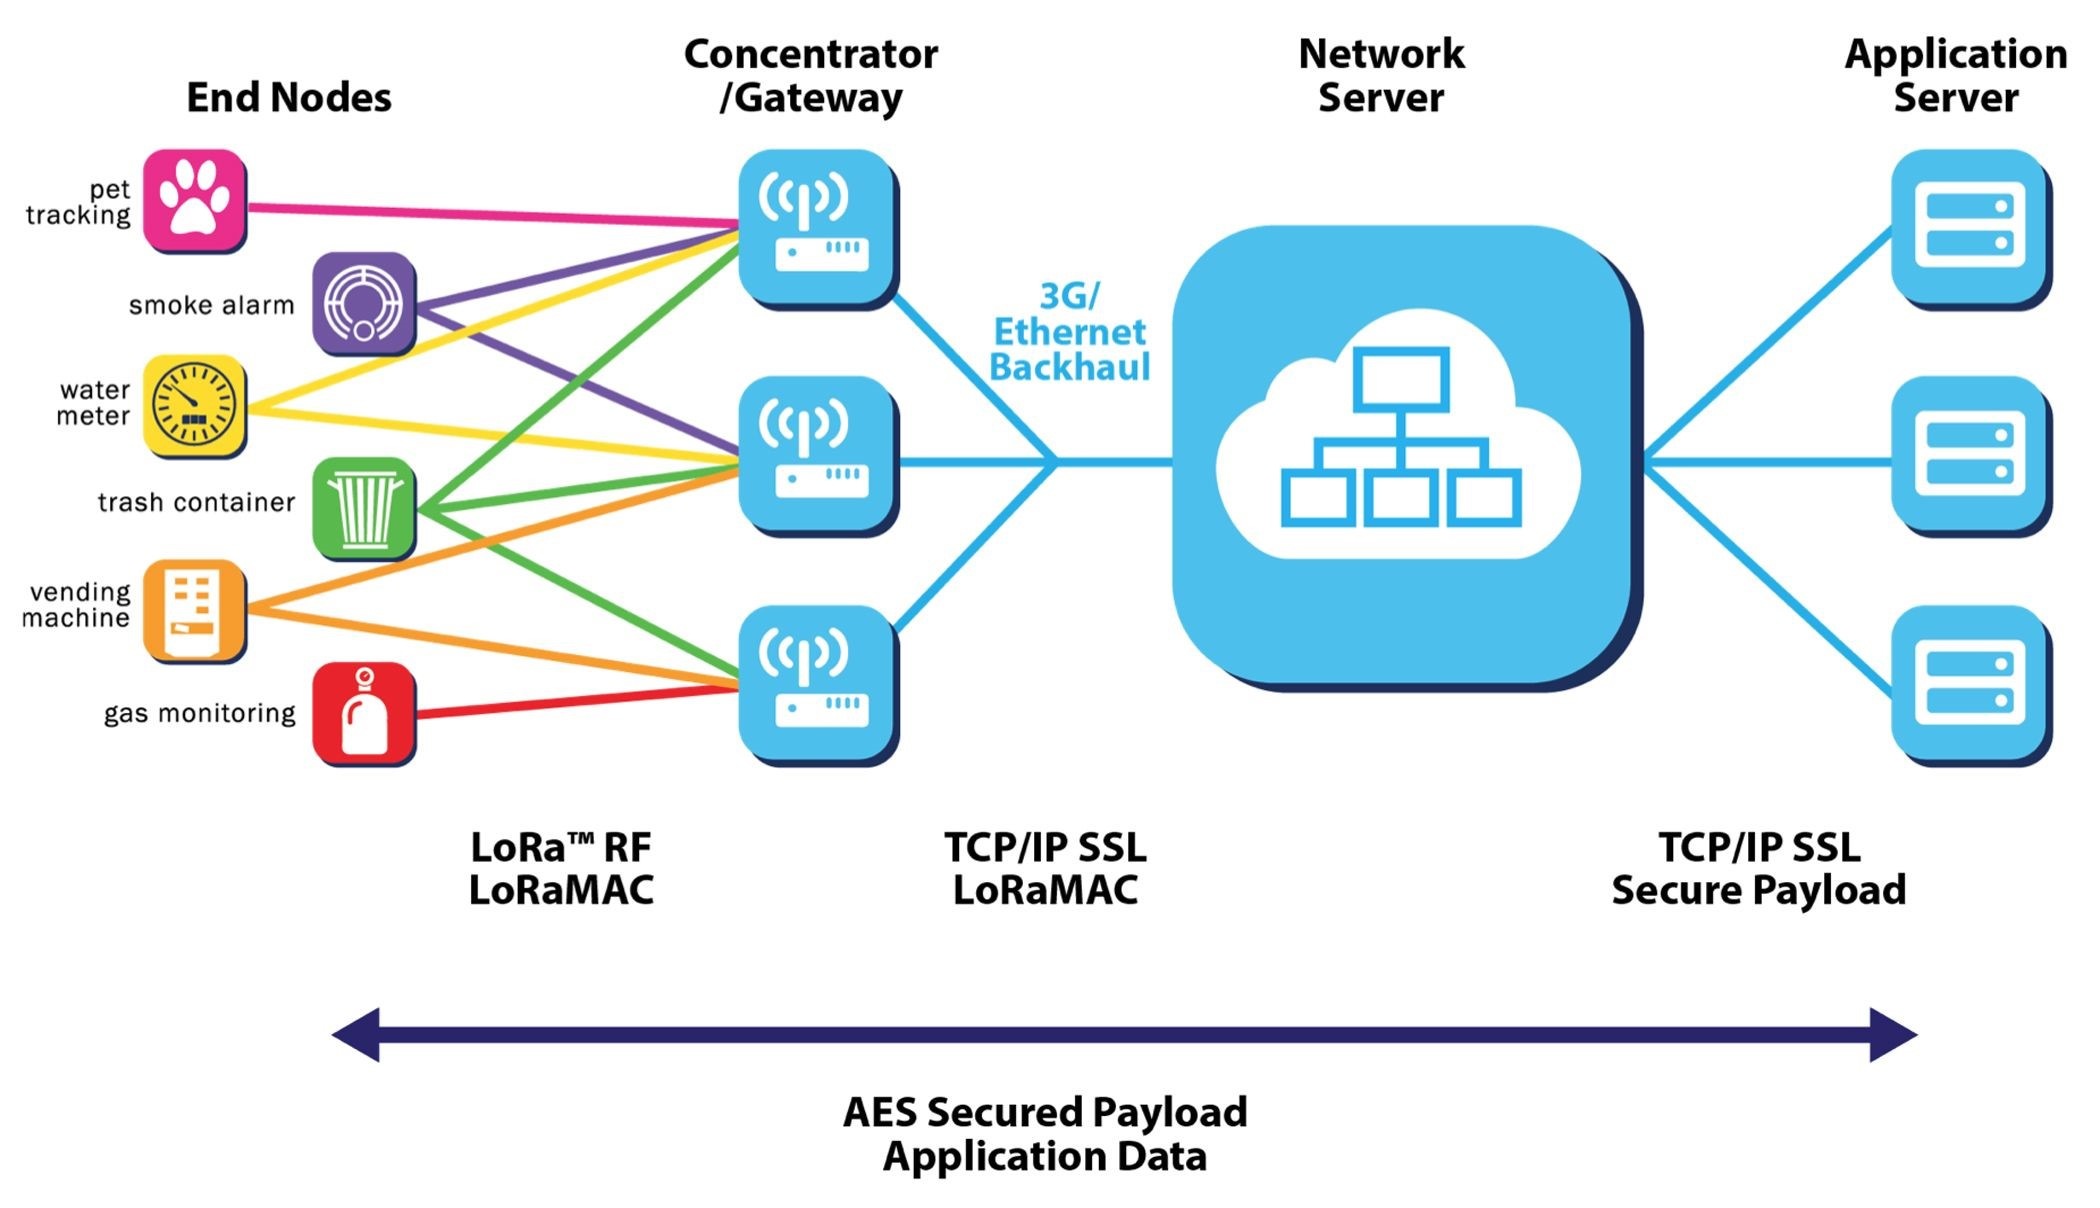
\includegraphics[width=0.7\textwidth]{figures/LoRa_Arch}
\caption{LoRa WAN Topology (taken from \cite{LoRaAlliance2015}).}\label{fig:loraarch}
\end{figure}

Due to the prime requirement of long range data transmission, field tests for LoRaWAN are mainly concerned with assessing signal strength and quality in dependence of the distance between device and gateway. There, different quality measures are studied (cf. \cite{Aref2014, Marais2017, }).
\begin{enumerate}
\item The Receiver Signal Strength Indicator (RSSI) ) is the total signal power received in milliwatts. The RSSI  is  measured  in  the  decibel-milliwatts  (dBm).
\item The Signal-to-Noise ratio (SNR) is  a  ratio  between  the  level  of  the  signal  and  the  level  of noise.
\item The packet-loss refers to frames that are not received by the network server. Such frames can be either not received at all by the gateway or received by the gateway but with a bad CRC (Cyclic Redundancy Check) so they can not be decoded.
\end{enumerate}

In this work we focus on the RSSI as quality measure of the network coverage. Under ideal conditions, the RSSI value has a logarithmic dependence on the distance $d$ of the device to the gateway, i.e.
\begin{equation}\label{eqn:loglaw}
\text{RSSI} = A -B \log_{10}(d)
\end{equation}
for some constants $A$ and $B$. In practice, however, the decay of signal strength also heavily depends on localized effects such as the surrounding elevation, environmental influences as well as buildings and vegetation that loom in the Fresnel zone of the device/gateway pair.   

In order to generate a reliable heat map that predicts the RSSI values between measurement points, we employ techniques from geospatial statistics (cf. \cite{Cressi1993, Webster2007}). In particular, we use regression kriging that allows for the spatial variance structure of the measurements and hence yields RSSI predictions that are sensitive to localized effects. In our situation, regression kriging amounts to update the predictions of the logarithmic regression model above with spatially interpolated residuals that take into account the covariance structure of the neighborhood of the spatial point under consideration.  

The constribution of this work is threefold:
\begin{enumerate}

\end{enumerate}

\bibliographystyle{abbrv}
\bibliography{literature}


\end{document}